\documentclass[12pt, a4paper]{article}

\usepackage[utf8]{inputenc}
\usepackage[T1]{fontenc}
\usepackage[spanish]{babel}
\usepackage{geometry}
\usepackage{graphicx}
\usepackage{hyperref}
\usepackage{listings}
\usepackage{xcolor}
\usepackage{enumitem}
\usepackage{titlesec}
\usepackage{fancyhdr}
\usepackage{parskip}

\geometry{margin=2.5cm}

\hypersetup{
    colorlinks=true,
    linkcolor=blue!70!black,
    urlcolor=blue!70!black,
    citecolor=blue!70!black,
}

\lstset{
    basicstyle=\ttfamily\small,
    keywordstyle=\color{blue!70!black}\bfseries,
    commentstyle=\color{green!50!black}\itshape,
    stringstyle=\color{red!60!black},
    breaklines=true,
    frame=single,
    backgroundcolor=\color{gray!10},
    numbers=left,
    numberstyle=\tiny\color{gray},
}

\pagestyle{fancy}
\setlength{\headheight}{15pt}
\fancyhf{}
\fancyhead[L]{\textit{Campus Eventos}}
\fancyhead[R]{\textit{Proyecto Flutter}}
\fancyfoot[C]{\thepage}
\renewcommand{\headrulewidth}{0.4pt}

\title{\textbf{Campus Eventos} \\ \large Aplicación de Consulta de Eventos Universitarios \\ \normalsize Desarrollo de Interfaz en Flutter}
\author{Andrew}
\date{\today}

\begin{document}

\maketitle
\thispagestyle{empty}

\newpage
\tableofcontents
\newpage

%% =====================================================================
\section{Introducción}
%% =====================================================================

El presente documento describe el desarrollo de \textbf{Campus Eventos}, una aplicación móvil construida con Flutter cuyo objetivo es permitir a los estudiantes universitarios consultar las diferentes actividades que se realizan dentro de la institución.

La aplicación ofrece una interfaz visualmente atractiva basada en la paleta de colores \textit{Gruvbox Dark}, organizada por categorías (Académicos, Deportivos, Culturales, Tecnología y Talleres), con un sistema de filtrado en tiempo real y diseño responsivo que se adapta a distintos tamaños de pantalla.

%% =====================================================================
\section{Desarrollo}
%% =====================================================================

\subsection{Estructura del proyecto}

El proyecto sigue una arquitectura limpia y organizada en carpetas temáticas dentro del directorio \texttt{lib/}:

\begin{lstlisting}[basicstyle=\ttfamily\small, frame=none, numbers=none]
lib/
+-- main.dart
+-- data/
    +-- event_data.dart
+-- screens/
    +-- home_page.dart
+-- widgets/
    +-- event_card.dart
    +-- category_chip.dart
+-- theme/
    +-- app_theme.dart
\end{lstlisting}

Cada carpeta tiene una responsabilidad clara: \texttt{data/} contiene los datos de los eventos, \texttt{screens/} alberga las pantallas principales, \texttt{widgets/} los componentes reutilizables y \texttt{theme/} la configuración visual de la aplicación.

\subsection{Widgets utilizados}

La aplicación utiliza los siguientes widgets de Flutter, cumpliendo con todos los requisitos de la práctica:

\begin{itemize}[noitemsep]
    \item \textbf{StatefulWidget}: \texttt{HomePage} como widget principal con estado.
    \item \textbf{setState()}: para actualizar la categoría seleccionada y re-renderizar la interfaz.
    \item \textbf{GridView.builder}: para mostrar los eventos en una cuadrícula adaptable.
    \item \textbf{Card}: como contenedor de cada evento en la tarjeta \texttt{EventCard}.
    \item \textbf{ListView.builder}: para el scroll horizontal de las categorías (chips de filtro).
    \item \textbf{ChoiceChip}: implementado en \texttt{CategoryChip} para la selección de categorías.
    \item \textbf{SnackBar}: para mostrar confirmación al presionar ``Me interesa''.
    \item \textbf{Image.network}: para cargar imágenes de los eventos desde la red.
    \item \textbf{Row / Column}: para la organización horizontal y vertical de los elementos.
\end{itemize}

Otros widgets complementarios incluyen \texttt{AppBar}, \texttt{SafeArea}, \texttt{Padding}, \texttt{LayoutBuilder}, \texttt{Expanded}, \texttt{Flexible} y \texttt{FilledButton.tonalIcon}.

\subsection{Funcionamiento general}

La aplicación inicia en \texttt{main.dart}, que ejecuta \texttt{CampusEventosApp}, un \texttt{StatelessWidget} que configura el \texttt{MaterialApp} con el tema personalizado Gruvbox y carga la pantalla principal \texttt{HomePage}.

La pantalla principal presenta:
\begin{enumerate}[noitemsep]
    \item Un encabezado con el título ``Eventos universitarios'' y una descripción general.
    \item Una lista horizontal de categorías filtrables mediante chips.
    \item Un contador de ``Eventos encontrados'' que se actualiza dinámicamente.
    \item Una cuadrícula de tarjetas de eventos que muestra imagen, nombre, categoría, fecha, hora, lugar y cupo de cada actividad.
    \item Un botón ``Me interesa'' en cada tarjeta que activa un SnackBar con el nombre del evento.
\end{enumerate}

%% =====================================================================
\section{Implementación}
%% =====================================================================

\subsection{Filtrado de eventos}

El filtrado se implementa en el método \texttt{build} de \texttt{HomePage}. La variable \texttt{categoriaSeleccionada} almacena la categoría activa y se evalúa con una expresión condicional:

\begin{lstlisting}[basicstyle=\ttfamily\small]
final eventosMostrados = categoriaSeleccionada == 'Todos'
    ? eventos
    : eventos.where((e) => e['categoria'] == categoriaSeleccionada).toList();
\end{lstlisting}

Cuando se selecciona ``Todos'', se muestran los 18 eventos. Al seleccionar una categoría específica, se filtra la lista usando \texttt{where()} y se muestra únicamente los eventos correspondientes. El contador de ``Eventos encontrados'' se actualiza automáticamente al usar la longitud de \texttt{eventosMostrados}.

\subsection{Manejo de estado}

El estado se gestiona de forma nativa con \texttt{StatefulWidget} y \texttt{setState}. La variable \texttt{categoriaSeleccionada} es el único campo de estado, lo cual es adecuado para la complejidad de esta aplicación. No se utilizaron paquetes externos de gestión de estado (Provider, BLoC, Riverpod), ya que el alcance del proyecto no lo requiere.

El flujo de datos sigue un patrón ascendente-descendente:
\begin{itemize}[noitemsep]
    \item Los datos (\texttt{evento}) y callbacks (\texttt{onPressed}) se pasan \textbf{hacia abajo} a \texttt{EventCard}.
    \item Las selecciones (\texttt{onTap}) se propagan \textbf{hacia arriba} al widget padre.
\end{itemize}

\subsection{Diseño responsivo}

La adaptación a distintos tamaños de pantalla se logra mediante \texttt{LayoutBuilder} en el cuerpo de la pantalla principal. Se definen tres breakpoints:

\begin{lstlisting}[basicstyle=\ttfamily\small]
int crossAxisCount;
if (constraints.maxWidth >= 900) {
  crossAxisCount = 4;
} else if (constraints.maxWidth >= 600) {
  crossAxisCount = 3;
} else {
  crossAxisCount = 2;
}
\end{lstlisting}

Adicionalmente, se utiliza \texttt{mainAxisExtent: 370} en el \texttt{SliverGridDelegateWithFixedCrossAxisCount} para garantizar que las tarjetas no se desborden en ningún ancho de pantalla. Los textos largos se manejan con \texttt{maxLines} y \texttt{TextOverflow.ellipsis}.

\subsection{Organización del código}

El proyecto se divide en cuatro capas claras:

\begin{itemize}[noitemsep]
    \item \textbf{Datos} (\texttt{event\_data.dart}): Lista constante de 18 eventos y 6 categorías, sin dependencias de widgets.
    \item \textbf{Pantallas} (\texttt{home\_page.dart}): Lógica de presentación y estado.
    \item \textbf{Widgets} (\texttt{event\_card.dart}, \texttt{category\_chip.dart}): Componentes reutilizables y modulares.
    \item \textbf{Tema} (\texttt{app\_theme.dart}): Paleta de colores Gruvbox completa y configuración de \texttt{ThemeData} con Material 3.
\end{itemize}

\subsection{Tema visual Gruvbox}

La propuesta visual propia se basa en la paleta de colores \textit{Gruvbox Dark}, una paleta popular en la comunidad de terminales y editores de código. Se implementó una clase \texttt{GruvboxPalette} con más de 30 colores estáticos y un \texttt{ColorScheme} personalizado de Material 3, aplicándose a \texttt{AppBar}, tarjetas, chips, botones y snack bars.

%% =====================================================================
\section{Resultados}
%% =====================================================================

A continuación se presentan capturas de pantalla de la aplicación funcionando en distintos tamaños de pantalla.

\begin{figure}[h!]
    \centering
    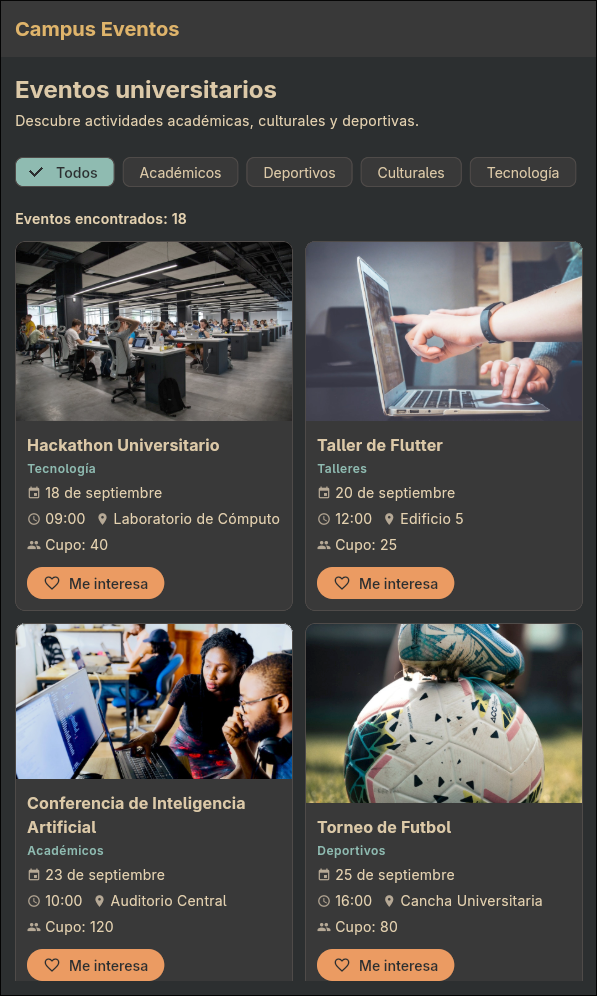
\includegraphics[width=0.42\textwidth]{screenshots/phone_mode(2-columns).png}
    \caption{Vista de la aplicación en dispositivo móvil (cuadrícula de 2 columnas).}
    \label{fig:mobile}
\end{figure}

\begin{figure}[h!]
    \centering
    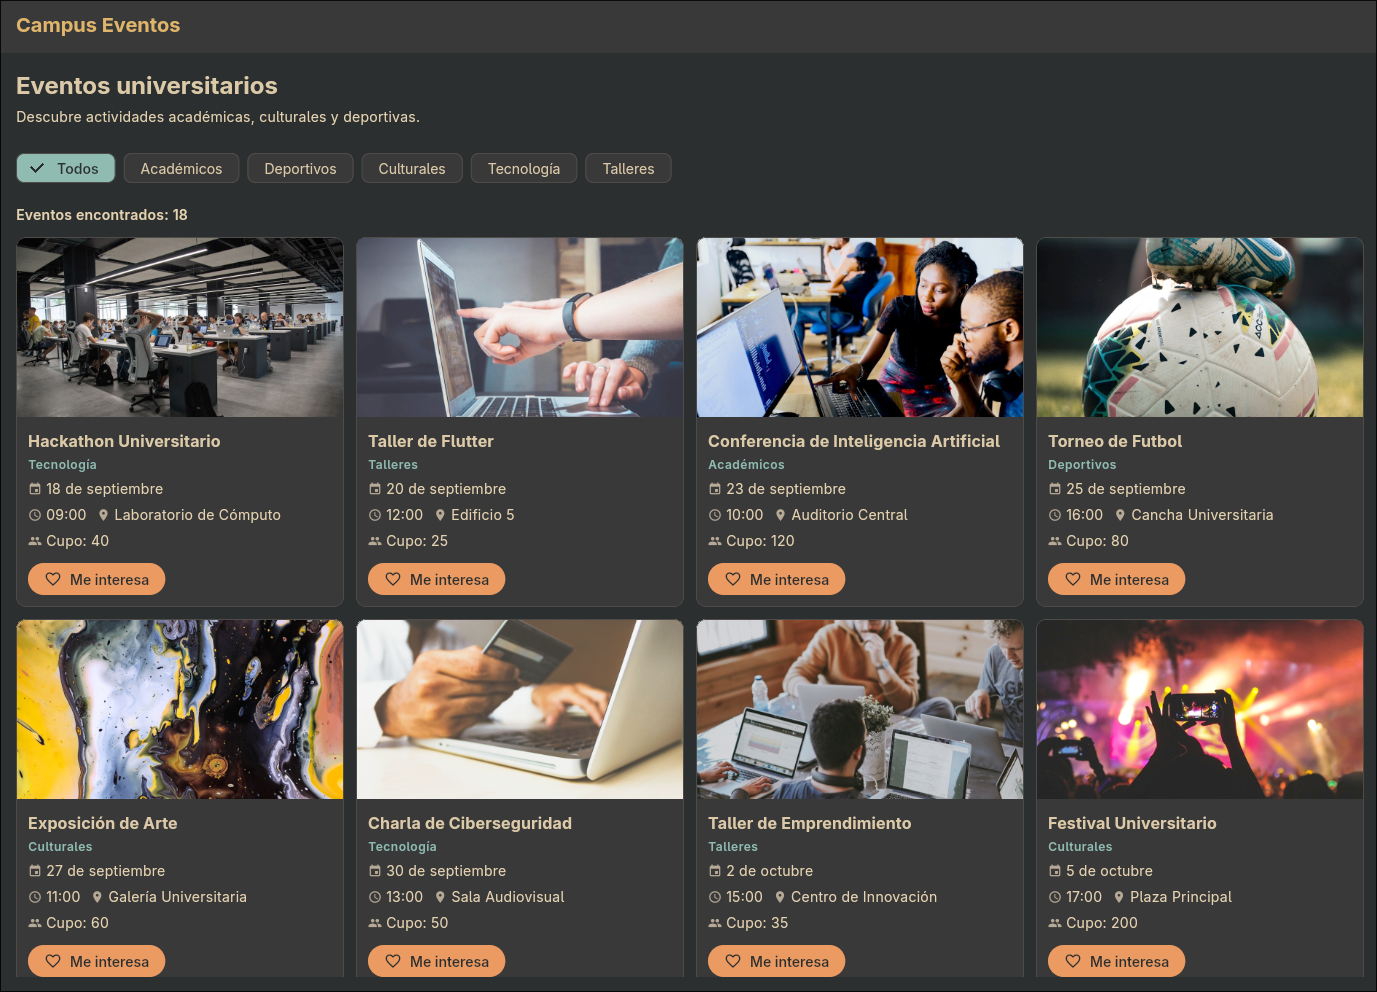
\includegraphics[width=0.85\textwidth]{screenshots/tablet_mode(4-columns).png}
    \caption{Vista de la aplicación en pantalla ampliada (cuadrícula de 4 columnas).}
    \label{fig:tablet}
\end{figure}

\begin{figure}[h!]
    \centering
    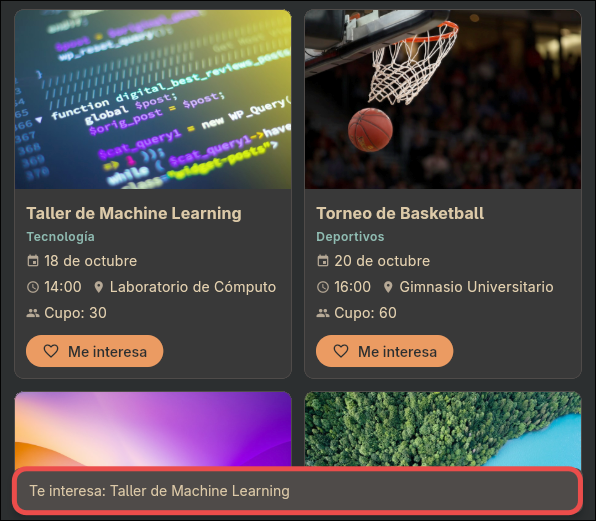
\includegraphics[width=0.42\textwidth]{screenshots/snackbar.png}
    \caption{SnackBar de confirmación al interactuar con un evento.}
    \label{fig:snackbar}
\end{figure}

\noindent Las capturas se obtuvieron ejecutando la aplicación en un dispositivo móvil y en una ventana ampliada de escritorio.

%% =====================================================================
\section{Conclusiones}
%% =====================================================================

\subsection{Aprendizajes}

Durante el desarrollo de esta práctica se consolidaron los siguientes conocimientos:

\begin{itemize}[noitemsep]
    \item Uso correcto de \texttt{StatefulWidget} y \texttt{setState} para la gestión de estado simple.
    \item Construcción de interfaces modulares mediante widgets reutilizables (\texttt{EventCard}, \texttt{CategoryChip}).
    \item Implementación de diseños responsivos con \texttt{LayoutBuilder} y breakpoints dinámicos.
    \item Organización del código en capas para mantener la separación entre datos, presentación y estilos.
    \item Creación de un tema visual personalizado con Material 3 y una paleta de colores externa.
    \item Manejo de imágenes de red con \texttt{errorBuilder} para evitar errores en pantalla.
\end{itemize}

\subsection{Problemas encontrados y soluciones}

\begin{enumerate}[noitemsep]
    \item \textbf{Desbordamiento de tarjetas en pantallas pequeñas:} Se solucionó fijando \texttt{mainAxisExtent: 370} en el delegado del \texttt{GridView}, garantizando que cada celda tenga una altura fija independiente del contenido.

    \item \textbf{Textos largos que rompían el diseño:} Se aplicó \texttt{maxLines} con \texttt{TextOverflow.ellipsis} en títulos y descripciones, junto con \texttt{Flexible} y \texttt{Expanded} para distribuir el espacio restante.

    \item \textbf{Fallo al cargar imágenes de red:} Se implementó un \texttt{errorBuilder} en \texttt{Image.network} que muestra un ícono de respaldo (\texttt{Icons.image\_not\_supported}) sobre un fondo de color cuando la imagen no está disponible.

    \item \textbf{Filtrado que no actualizaba el contador:} Se verificó que el contador ``Eventos encontrados'' estuviera referenciando la lista ya filtrada (\texttt{eventosMostrados.length}) y no la lista completa.

    \item \textbf{Color del texto en chips de categoría:} Se ajustó el tema de \texttt{ChoiceChip} en \texttt{AppTheme} para asegurar la legibilidad del texto sobre el fondo seleccionado, resolviendo un problema de contraste con la paleta Gruvbox.
\end{enumerate}

%% =====================================================================
\section{Anexos}
%% =====================================================================

\subsection{Repositorio del proyecto}

El código fuente completo de la aplicación está disponible en GitHub:

\url{https://github.com/Andrew869/flutter-app-eventos}

\subsection{Tecnologías utilizadas}

\begin{itemize}[noitemsep]
    \item \textbf{Flutter SDK}: Framework de desarrollo multiplataforma.
    \item \textbf{Dart}: Lenguaje de programación.
    \item \textbf{Material Design 3}: Sistema de diseño visual.
    \item \textbf{Paleta Gruvbox Dark}: Esquema de colores personalizado.
\end{itemize}

\subsection{Categorías y eventos}

\begin{table}[h!]
    \centering
    \begin{tabular}{|l|c|}
        \hline
        \textbf{Categoría} & \textbf{Número de eventos} \\
        \hline
        Todos & 18 \\
        Académicos & 3 \\
        Deportivos & 3 \\
        Culturales & 4 \\
        Tecnología & 4 \\
        Talleres & 4 \\
        \hline
    \end{tabular}
    \caption{Distribución de eventos por categoría.}
    \label{tab:eventos}
\end{table}

\end{document}
